\chapter{Complex Numbers}
This chapter is based on the following sources: \cite{complexpaul}, \cite{complexpurple}, \cite{complexnotebook}.
\\
\noindent 
The following chapter will first describe the concept of complex numbers and how to operate them mathematically. Additionally, it will introduce complex numbers in polar coordinates and the complex exponential function. %Complex numbers is needed when explaining the Laplace transform.
\\\\
\noindent 
When using real numbers, you cannot always solve a given equation. An example of this could be the equation $x^2=-1$. To solve this equation, the imaginary unit is introduced. The imaginary unit is defined as:
\begin{align*}
i=\sqrt{-1}.
\end{align*}
When $i$ is raised to a power greater than one, it becomes:
\begin{align*}
i^2=-1,\  i^3=-i,\  i^4=1.
\end{align*}

\noindent If $i$ is raised to a power greater than four, it will loop through the same values: $i, \ -1, \ -i$ and $1$. This can be expressed algebraically. Let $n$ be a positive integer. 
\\
Since: $$i^{4n} = i^4i^4\cdots i^4 = 1,$$
the greater exponents of $i$ become:
\begin{align*}
	i^{4n+1} =& i^{4n}i^1 = i, \\
	i^{4n+2} =& i^{4n}i^2 = -1, \\
	i^{4n+3} =& i^{4n}i^3 = -i, \\
	i^{4n+4} =& i^{4n}i^4 = 1.
\end{align*}
Complex numbers are denoted as $z = a+ib$, where $a,b\in \R$. A complex number consists of a real part and an imaginary part. The real and imaginary part of a complex number is written as $\text{Re}\{z\}=a$ and $\text{Im}\{z\}=b$, respectively.
An example of a complex number could be: $z=7+5i$, where 7 is the real part, and 5 is the imaginary part. 
\\
If $\text{Re}\{z\}=0$, the number is said to be purely imaginary.  
\\\\
Complex numbers are plotted in the complex plane. The complex plane consists of two axes: one real along the horizontal axis and an imaginary along the vertical axis.\\
The length from the origin to the complex number is called the modulus or the absolute value of the number.

\begin{definition}{Modulus of a complex number}{modulus}
The modulus of a complex number $z=a+ib$ is:
$$\mid z\mid=\sqrt{a^2+b^2}.$$
\end{definition}
\noindent
Every complex number has a complex conjugate. The conjugate of a complex number has the same real part, but the imaginary part has opposite sign.
\\

\begin{definition}{Complex number conjugated}{}
The complex conjugate of $z=a+ib$ is given by:
$$\bar{z}=a-ib.$$
\end{definition}

\noindent An example is shown in the figure below.  

\begin{figure}[H]
\centering
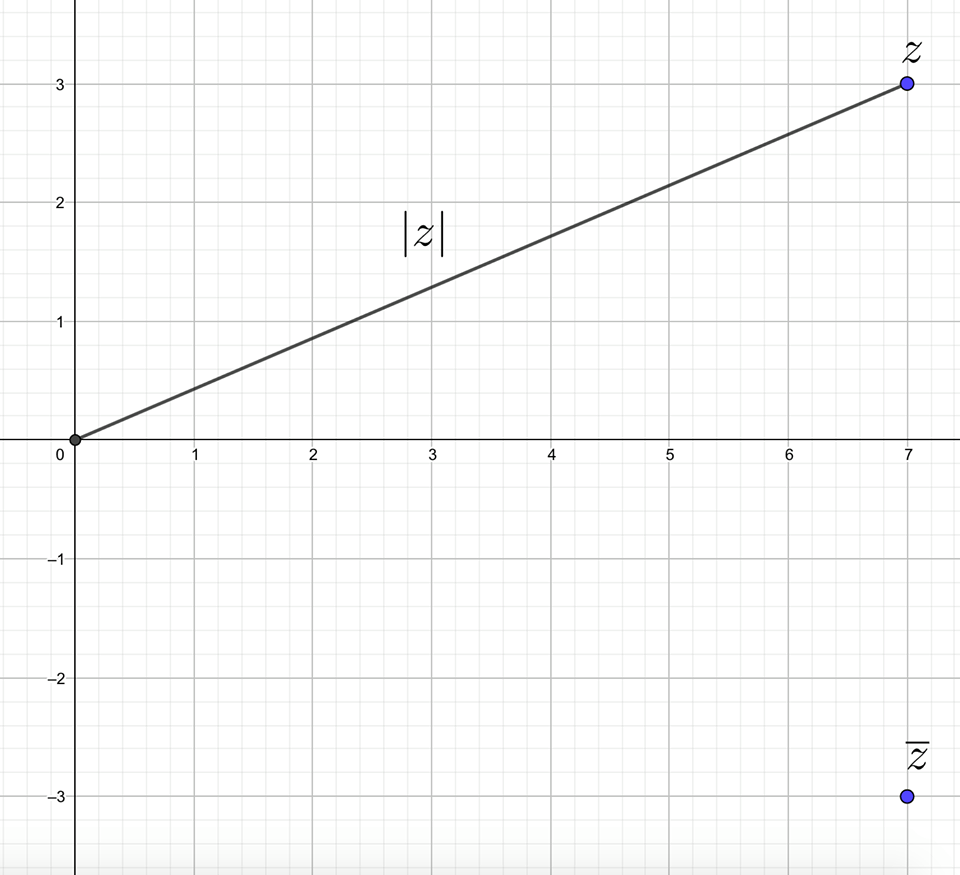
\includegraphics[scale=0.2]{fig/img/complex_plan}
\caption{The complex plane with the number $z=7+5i$, its conjugate $\bar{z}=7-5i$, and \  $|z|=8.6$.}
\end{figure}


\section{Addition and subtraction}
When adding complex numbers, the imaginary unit $i$ can be treated as a constant, as with elementary algebra:
\begin{align*}
(a + bi) + (c + di) = (a + c) + i(b + d).
\end{align*} 
\begin{example}{Addition}{}
Addition of two complex numbers:
\begin{align*}
(5+2i)+(9+8i)=14+10i.
\end{align*}
\end{example}


\noindent 
Subtraction has the general form:
\begin{align*}
(a + bi) - (c + di) = (a - c) + i(b - d),
\end{align*}
where the imaginary part can be subtracted with another imaginary part, and the real parts from the other real parts.

\begin{example}{Subtraction}{}
Subtraction of two complex numbers:
\begin{align*}
(21 + 3i) - (2 - 2i) = 21 + 3i - 2 + 2i = 19 + 5i.
\end{align*}
\end{example}

\section{Multiplication}
When multiplying complex numbers, the fact that $i^2 =-1$ must be taken into account. However, multiplication of complex numbers can still be generalized. 
\begin{definition}{Multiplying complex numbers}{def:MCN}
The product of two complex numbers $z_1=a+ib$ and $z_2=c+id$ has the general form:
\begin{align*}
(a+ib)(c+id)&=a(c+id)+ib(c+id),
\\
&=ac+iad+ibc+i^2bd,
\\
&=(ac-bd)+i(ad+bc).
\end{align*}
\end{definition}
\begin{example}{Multiplying complex numbers}{}
Given two complex numbers $z_1=3+5i$ and $z_2=4-3i$, the product can be found using \cref{def:MCN}:
\begin{align*}
(3+5i)(4-3i) = \big(3\cdot4-5\cdot(-3)\big)+i\big(3\cdot(-3)+5\cdot4\big)=27+11i.
\end{align*}
\end{example}


\section{Division}
The division between complex numbers can be difficult to visualize, without them being in the form: $a + ib$. 
\begin{definition}{Dividing complex numbers}{def:DCM}
Division of two complex numbers, where $z_1=a+ib$ and $z_2=c+id$, has the general form:
\begin{align*}
\frac{a + ib}{c + id} = \frac{(a+ib)(c-id)}{(c+id)(c-id)}.
\end{align*}
By using \cref{def:MCN} on the numerator, it becomes:  
\begin{align*}
\frac{(a+ib)(c-id)}{(c+id)(c-id)} &= \frac{(ac+bd)+i(bc-ad)}{c^2+d^2},							\\[1em]
&= \frac{ac+bd}{c^2+d^2}+i \frac{bc-ad}{c^2+d^2}.				
\end{align*}
\end{definition}
\begin{example}{Dividing complex numbers}{}
Given two complex numbers $z_1=18+10i$ and $z_2=3+2i$, the division can be found using \cref{def:DCM}:
\begin{align*}
\frac{18 + 10i}{3 + 2i} &= \dfrac{18\cdot3+10\cdot2}{3^2+2^2}+i\dfrac{10\cdot3-18\cdot2}{3^2+2^2},
\\
&=\dfrac{74}{13}-\dfrac{6}{13}i.
\end{align*}
\end{example}


\noindent From the example, $\dfrac{74}{13} - \dfrac{6}{13}i$ is now on the form $a+ib$ with $a$ and $b$ being fractions. In the example, the denominator is conjugated. As a result, the imaginary part of the denominator $ib$ disappears, and is only left in the numerator. 


\section{Complex numbers in polar form}

\begin{definition}{Complex number in polar form}{}
A complex number $z=a+ib$ can be written in polar form as follows:
\begin{align*}
z&=r\cos(\theta)+ir\sin(\theta),
\\
&=r\big(\cos(\theta)+i\sin(\theta)\big),
\end{align*}
where $r=\mid z \mid$ and $\theta=\tan^{-1}\left(\dfrac{b}{a} \right).$
\end{definition}

\noindent A complex number $z=a+ib$ can be written is polar form as $\big(r,\theta\big)$, where $r$ is the distance from the origin to the point $z$ and $\theta$ is the angle from the real axis to $r$, when measured counter-clockwise. The angle of a complex number is denoted as $\arg(z)=\theta$. This is shown in the figure below.
\begin{figure}[H] 
\centering
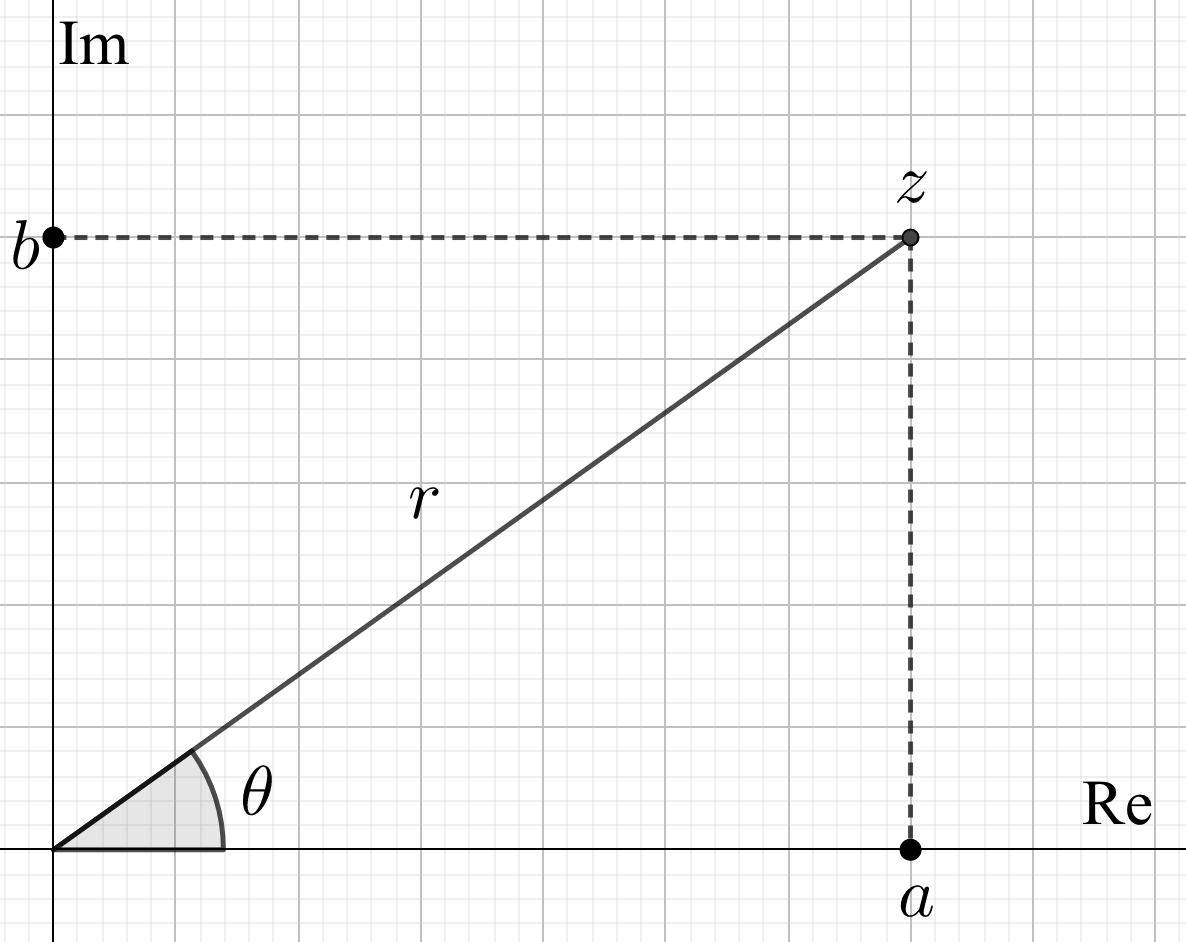
\includegraphics[scale=0.15]{fig/img/complex_plan_polar}
\caption{The complex plane with $z=a+ib$ plotted in terms of polar coordinates and Cartesian coordinates.}
\label{fig:complex_plane_polar}
\end{figure}
\noindent
From figure \ref{fig:complex_plane_polar}, the coordinates of $z=a+ib$ can be expressed as follows:
\begin{align}
a=\text{Re}\{z\}=r\cos(\theta),
\\
b=\text{Im}\{z\}=r\sin(\theta).
\end{align}
\\

\begin{theorem}{Multiplication in polar form}{complex:multi}
Given two complex numbers $z_1$ and $z_2$, where:
\begin{align*}
z_1=r_1\big( \cos(\theta_1)+i\sin(\theta_1) \big), 
\\
z_2=r_2\big( \cos(\theta_2)+i\sin(\theta_2) \big),
\end{align*}
the multiplication of these are given by:
\begin{align}
z_1 z_2=r_1r_2\big( \cos(\theta_1+\theta_2)+ i \sin(\theta_1+\theta_2)\big). \label{pol:trig}
\end{align}
\end{theorem}


\begin{prof}{}{the:multi_polar}
%Kristian vil have noget tekst i stedet for vi går direkte igang med en ligning
\begin{align}
z_1 z_2&=r_1 \big( \cos(\theta_1)+ i \sin(\theta_1)\big)r_2 \big( \cos(\theta_2)+ i \sin(\theta_2)\big), \nonumber
\\
\label{polar_multiplication}
z_1z_2&=r_1r_2\Big( \big(\cos(\theta_1)\cos(\theta_2)-\sin(\theta_1) \sin(\theta_2)\big)+i\big(\cos(\theta_1)\sin(\theta_2)+\sin(\theta_1)\cos(\theta_2)\big)\Big).
\end{align}
By definition, the sine and cosine of the sum of two angles, can be written as follows: \cite[p. A-14 Appendicies]{calc}
\\
\begin{align} 
\sin(\theta_1+\theta_2)=\cos(\theta_1)\sin(\theta_2)+\sin(\theta_1)\cos(\theta_2), \label{sum_cos_sin}
\end{align}
\begin{align*}
\cos(\theta_1+\theta_2)=\cos(\theta_1)\cos(\theta_2)-\sin(\theta_1)\sin(\theta_2).
\end{align*}
\\
These definitions are inserted in \eqref{polar_multiplication}:
\\
\begin{align*}
z_1 z_2=r_1r_2\big( \cos(\theta_1+\theta_2)+ i \sin(\theta_1+\theta_2)\big).
\end{align*}
\end{prof}
\noindent
From  \eqref{the:multi_polar}, the following relation can be found:
\begin{align}
\arg(z_1z_2)&=\arg(z_1)+\arg(z_2),
\\
|z_1z_2|&=|z_1||z_2|.
\end{align}

\begin{theorem}{Division in polar form}{the:div_polar}
Given two complex numbers:
\begin{align*}
z_1=r_1\big(\cos(\theta_1)+i\sin(\theta_1)\big), 
\\
z_2=r_2\big(\cos(\theta_2)+i\sin(\theta_2)\big),
\end{align*}
the division of these are given by:
\begin{align*}
\dfrac{z_1}{z_2}=\dfrac{r_1}{r_2}\Big( \cos(\theta_1-\theta_2)+ i \sin(\theta_1-\theta_2)\Big).
\end{align*}
\end{theorem}


\begin{prof}{}{}
\begin{align*}
\dfrac{z_1}{z_2}&=\dfrac{r_1\Big(\cos(\theta_1)+i\sin(\theta_1)\Big)}{r_2\Big(\cos(\theta_2)+i\sin(\theta_2)\Big)}.
\end{align*}
The numerator and the denominator on the right side are multiplied by $r_2\Big(\cos(\theta_2)-i\sin(\theta_2)\Big)$:
\begin{align*}
\dfrac{z_1}{z_2}&=\dfrac{r_1\Big(\cos(\theta_1)+i\sin(\theta_1)\Big)r_2\Big(\cos(\theta_2)-i\sin(\theta_2)\Big)}{r_2\Big(\cos(\theta_2)+i\sin(\theta_2)\Big)r_2\Big(\cos(\theta_2)-i\sin(\theta_2)\Big)},
\\
&=\dfrac{r_1 r_2}{r_2^2}  \dfrac{\cos(\theta_1)\cos(\theta_2)-i\cos(\theta_1)\sin(\theta_2)+i\sin(\theta_1)\cos(\theta_2)+sin(\theta_1)\sin(\theta_2)}{\cos^2(\theta_2)-i\sin(\theta_2)\cos\theta_2)+i\sin(\theta_2)\cos\theta_2)+\sin^2(\theta_2)}.
\end{align*}
Since the sine and cosine of the difference between two angles are defined as:
\begin{align*}
\cos(\theta_1-\theta_2)=\cos(\theta_1)\cos(\theta_2)+\sin(\theta_1)\sin(\theta_2),
\\
\sin(\theta_1-\theta_2)=\sin(\theta_1)\cos(\theta_2)-\cos(\theta_1)\sin(\theta_2),
\end{align*}
the equation can now be rewritten as:
\begin{align*}
\dfrac{z_1}{z_2}=\dfrac{r_1}{r_2}  \dfrac{\cos(\theta_1-\theta_2)+i\sin(\theta_1-\theta_2)}{\cos^2(\theta_2)+\sin^2(\theta_2)}.
\end{align*}
From the fundamental trigonometric identity: 
\begin{align*}
\cos^2(\theta)+\sin^2(\theta)=1.
\end{align*}
The equation can now be written as:
\begin{align*}
\dfrac{z_1}{z_2}&=\dfrac{r_1}{r_2}\Big( \cos(\theta_1-\theta_2)+ i \sin(\theta_1-\theta_2)\Big).
\end{align*}
\end{prof}
\noindent From \cref{the:div_polar}, the following relations can be derived:
\begin{align}
\arg\Big(\dfrac{z_1}{z_2}\Big)&=\arg(z_1)-\arg(z_2),
\\
\Big|\dfrac{z_1}{z_2}\Big|&=\dfrac{|z_1|}{|z_2|}. \label{eq:mod_div}
\end{align}

\section{The complex exponential function}
The concept of the complex exponential function is useful in circuit analysis. However, it must be defined, as it is not entirely obvious what $e$ raised to a complex number means.

\begin{definition}{Euler's identity}{eulers_form}
Euler's identity is defined as: \cite[p.~231]{diffandcomplex}
\begin{align}
e^{i\theta}=\cos(\theta)+ i \sin(\theta).
\end{align} 
\end{definition}
\begin{theorem}{Modulus of Euler's identity}{the:euler_form}
Modulus of $e^{i\theta}$ is said to be equal to one, for all $\theta \in \mathbb{R}$:
\begin{align*}
|e^{i\theta}|=1.
\end{align*}
\end{theorem}
\begin{prof}{}{}
Given the exponential:
\begin{align*}
z=e^{i\theta}=\cos(\theta)+i\sin(\theta),
\end{align*}
modulus of $z$ is defined as:
\begin{align}
|z|=\sqrt{\text{Re}\{z\}^2+\text{Im}\{z\}^2}, \label{eq:mod_euler}
\end{align}
where $\text{Re}\{z\}=\cos(\theta)$, and $\text{Im}\{z\}=\sin(\theta)$. This is inserted in \eqref{eq:mod_euler}:
\begin{align*}
|z|=|e^{i\theta}|=\sqrt{\cos^2(\theta)+\sin^2(\theta)}=\sqrt{1}=1.
\end{align*}
\end{prof}
\noindent In order for the complex exponential function to be useful in this context, it needs to fulfill two conditions:
\begin{itemize}
	\item $e^{z_1}e^{z_2} = e^{z_1 + z_2}$
	\item $\dfrac{d}{dt}e^{z} = ze^{z}$
\end{itemize}
The complex exponential function can be defined as follows, and it can be shown that this definition will satisfy the given conditions.
\\

\begin{definition}{The complex exponential function}{complex:exp:eq}
The complex exponential function is defined as:
\begin{align*}
	e^{z}=e^{a+ib}=e^{a}e^{ib}.
\end{align*}
\end{definition}

\noindent
Given this definition of the complex exponential function, it will then be shown that the conditions set earlier will hold.\\

\begin{theorem}{Multiplication of complex numbers in exponential form}{}
Given two complex numbers in exponential form $e^{z_1}$ and $e^{z_2}$ where:
\begin{align*}
z_1=a_1+ib_1,
\\
z_1=a_2+ib_2.
\end{align*}
The product of the two complex numbers is given by:
\begin{align*}
e^{z_1}e^{z_2}=e^{z_1+z_2}.
\end{align*}
\end{theorem}


\begin{prof}{}{proof:complex:exp:multi}
From \cref{complex:exp:eq}, the product can be written as:
\begin{align*}
e^{z_1}e^{z_2}&=e^{a_1}\big(\cos(b_1)+i\sin(b_1)\big)e^{a_2}\big(\cos(b_2)+i\sin(b_2)\big),
\\
&=e^{a_1}e^{a_2} \Big( \big(\cos(b_1)\cos(b_2)-\sin(b_1) \sin(b_2) \big)+i \big(\cos(b_1)\sin(b_2)+\sin(b_1)\cos(b_2) \big) \Big).
\end{align*}
From \eqref{sum_cos_sin}, this can be rewritten as:
\begin{align*}
e^{z_1}e^{z_2}=e^{a_1}e^{a_2}\big(\cos(b_1+b_2)+i(\sin(b_1+b_2)\big).
\end{align*}
Since both $e^{a_1}$ and $e^{a_2}$ are real numbers, their exponents can be added:
\begin{align*}
e^{z_1}e^{z_2}=e^{a_1+a_2}\big(\cos(b_1+b_2)+i(\sin(b_1+b_2)\big).
\end{align*}
From definition \cref{complex:exp:eq},
this can be rewritten as:
\begin{align*}
e^{z_1}e^{z_2}&=e^{a_1+a_2}e^{i(b_1+b_2)},
\\
&=e^{a_1+ib_1}e^{a_2+ib_2},
\\
&=e^{z_1+z_2}.
\end{align*} 
\end{prof}

\begin{theorem}{Differentiating a complex exponential function}{theorem:complex:exp}
Given the complex function:
\begin{align*}
f(t)=e^{zt}=e^{at}(\cos(bt)+i\sin(bt)),
\end{align*}
where $z=a+ib$ and $t\in \R$. The differentiation of $f$ with respect to $t$, is given by:
\begin{align*}
\dfrac{d}{dt}f(t)=ze^{zt}.
\end{align*}
\end{theorem}

\begin{prof}{}{proof:complex:diff:exp}
To show that the function $f(t)=e^{z t}$ is differentiable, where $z=a+ ib$:
\begin{align*}
	f(t) = e^{zt}= e^{(a+ib)t}= e^{at}  e^{ib t}.
\end{align*}
The imaginary part of the complex number $e^{ib\cdot t}$ can be rewritten using \cref{eulers_form}:
\begin{align*}
	f(t) =& e^{at}\big(\cos(bt)+i \cdot \sin(bt)\big), \\
		 =& e^{at}\cos(bt) + e^{at} i \cdot \sin(bt).
\end{align*}
The rewritten function can be differentiated using the chain rule:
\begin{align}
	\dfrac{d}{dt}f(t) =& ae^{at}\cos(bt) -ib \cdot \sin(bt)e^{at} + ia \cdot e^{at}\sin(bt) + ib \cdot e^{at}\cos(bt), \nonumber \\
	=& e^{at} \bigg( a\big(\cos(bt) + i \cdot \sin(bt)\big) + b\big(i \cdot \cos(bt) - \sin(bt)\big) \bigg), \nonumber \\
	=& e^{at}\bigg(a \cdot e^{ib \cdot t}+b\big(i \cdot \cos(bt) - \sin(bt)\big)\bigg), \nonumber \\
	=& a e^{t(a+ib)} + b e^{at}\big(i \cdot \cos(bt) - \sin(bt)\big). \label{proof:chain}
\end{align}
Since $i^2 = -1$, \eqref{proof:chain} can be rewritten. Furthermore, $a+ib$ is replaced with $z$:
\begin{align*}
	\dfrac{d}{dt}f(t) =& a e^{zt} + b e^{at}\big(i \cdot \cos(bt) + i^2 \cdot \sin(bt)\big).
\end{align*}
$i$ is now moved outside the parentheses, and \cref{eulers_form} is used to reduce the equation:
\begin{align*}
	\dfrac{d}{dt}f(t) =&  a e^{zt} + ib e^{at}\big(\cos(bt) + i \cdot \sin(bt)\big), \\
	=&  a e^{zt} + ib e^{at}e^{ib \cdot t}. \\
\end{align*}
Now $a+ib$ is replaced with $z$, and $e^{zt}$ can be placed outside of the parentheses:
\begin{align*}
	\dfrac{d}{dt}f(t) =&  a e^{zt} + ib e^{t(a+ib)}, \\
	=&  e^{zt}(a+ib).
\end{align*}
$a+ib$ is again replaced with $z$, and \cref{theorem:complex:exp} is proved.
\end{prof}


\noindent
It can now be concluded that both of the conditions stated at the beginning of this section are satisfied. 